\chapter{Neural Networks}
\begin{quotation}
\noindent ``\emph{quote}''
\begin{flushright}\textbf{auteur, date}\end{flushright}
\end{quotation}

\vspace*{0.5cm}


Neural networks have been very popular in the reinforcement learning community,
either to directly approximate policy functions or to approximate functions that
estimate the value of states and actions.\\

\section{Feedforward neural networks}
A neural network is a collection of interconnected \textit{neurons}. The
simplest and most widely used networks are feedforward neural networks. In this
setting, neurons are arranged into ordered layers of which the first one is
called the input layer, and the last one is called the output layer.
The first possible way of using neural networks for reinforcement learning
is to feed the observed state of the environment to the input layer, and to
use the normalised output of the network as a policy (a probability distribution
over the actions set).

\begin{figure}[]
	\centering
	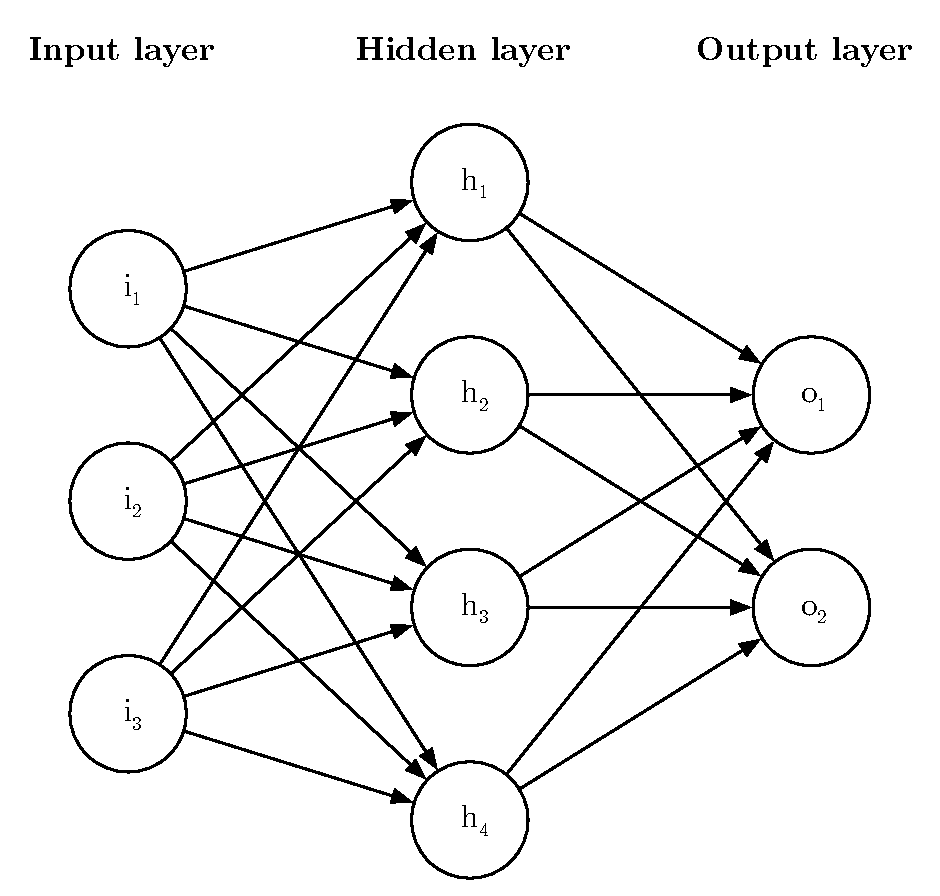
\includegraphics[width=0.6\linewidth]{fig/neural_network.eps}
	\caption{A neural network with one input layer composed of three neurons,
	one hidden layer of 4 neurons, and one output layer with 2 neurons.}
	\label{fig:neural_network}
\end{figure}


In a feedforward neural network, each neuron is connected to every neuron in 
the next layer.  To obtain an output from a given input,
the information will be passed from layer to layer in the following way : 
each neuron computes a weighted sum of the outputs of all neurons in the
previous layer then squashes this weighted sum in an activation function. 
Hence, the neuron $h_1$ in the network of Figure~\ref{fig:neural_network}
outputs:
$$ f(w_1i_1 + w_2i_2 + w_3i_3 + b) $$
where $w_1, w_2, w_3$ are the weights corresponding to the connections between
$i_1, i_2, i_3$ and $h_1$; and $b$ is a bias term. 
These weights are the learnable parameters of any neural network and will be 
tuned during training to improve the accuracy of the network. 
The activation function $f(\cdot)$ can be chosen arbitrarily, as long as it 
is differentiable (so that backpropagation can work, see \ref{nn:training})
but it is the same for all the neurons in the same layer. Some options are
the sigmoid function, the hyperbolic tangent function and sometimes a linear
function.\\

The reader might have noticed that using matrices is an efficient way of writing
and executing computations within a neural network. Indeed, one could write
the computation between the input layer and the first hidden layer as: 

$$ h = f(iW_{ih} + b_h) $$

\noindent where : 
\begin{itemize}
	\item $h$ is a $1\times n$ vector containing the values of the neurons 
		in the hidden layer
	\item $i$ is a $1\times m$ vector containing the values of the neurons
		in the input layer
	\item $W_{ih}$ is a $m\times n$ matrix containing the weights between
		the input and hidden layer
	\item $b_h$ is the $1\times n$ bias vector 
\end{itemize}

\subsection{Training}
\label{nn:training}
A neural network is taught to approximate a function on a training
set of samples. Learning is performed by alternating feedforward passes and 
backpropagation, modifiying the weights of the connections between neurons until
the network reaches a satisfying accuracy.

\begin{enumerate}
	\item the feedforward pass computes the network output from the sample
		input data
	\item the network output is compared with the sample output and the
		error signal given by a loss function
		is backpropagated through the network, updating
		all the weights
\end{enumerate}

Hence the importance of a \textbf{loss function} \index{loss function}
which describes numerically the error between the target and the network output.
This loss function has to be differentiable so that its gradient can be 
backpropagated through all the neurons in the network in order to 
minimise the error and nudge the network towards a behaviour we want it to
display.\\

Backpropagation uses the fact that activation functions are differentiable to
perform gradient descent. Indeed, the error signal is a surface in a space
of which the dimensionality is equal to the number of parameters in the
network. Gradient descent aims to find the global minimum of this error
surface.\\

\todo{Explain backprop?}


\section{Recurrent neural networks}
There is one limitation to feedforward neural networks which is particularly
critical for reinforcement learning applications. In many environments, the
present state does not carry enough information for the agent to make an
optimal decision. History and memory are necessary and cannot exist within
the framework of feedforward neural networks -- unless by inputting a fixed
number of previous states along with the present state. This approach however
limits the scope of the memory but also increases dramatically the complexity
of the model.\\

One solution to this problem is the use of recurrent neural networks.
A feedback loop such as the one shown in Figure~\ref{fig:rnn}a, also called
a recurrent connection, means that the layer at the receiving end of the
recurrent connection will receive as input not only the value of the previous
layer at time $t$, but also the value of the layer at the giving end of the 
recurrent connection at time $t-1$. This allows information to \textit{live}
throughout time steps.\\

A recurrent connection, however, poses evident issues for the backpropagation
algorithm since the depth of the neural network can become theoretically
infinite.  A common way of training and visualising recurrent neural networks 
is to unroll them for a given, finite amount of time steps (see 
Figure~\ref{fig:rnn}b).  The error signal can then be computed
for the output value at each time step, and backpropagated through all the
previous input values that affected its computing.\\

\begin{figure}[]
	\centering
	\subfloat[][A recurrent connection]{\qquad
		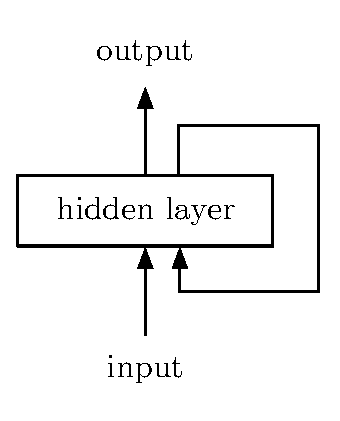
\includegraphics[width=0.1515\linewidth]{fig/recurrent_neural_network.eps}\qquad}
	\qquad
	\subfloat[][An unrolled recurrent neural network]{
		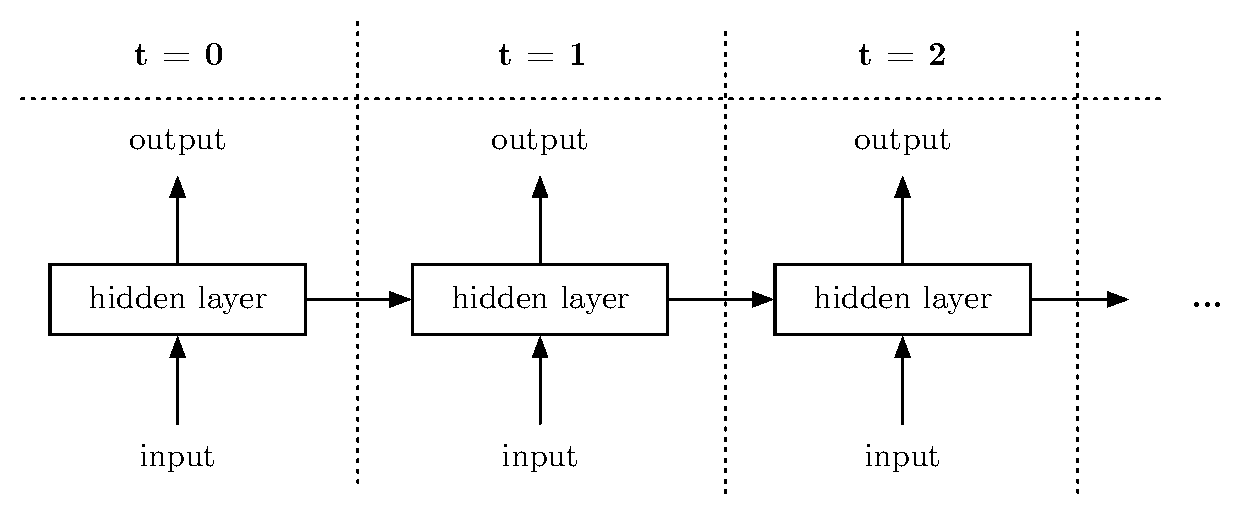
\includegraphics[width=0.6\linewidth]{fig/recurrent_neural_network_unrolled.eps}}
	\caption{Recurrent neural networks}
	\label{fig:rnn}
\end{figure}

\todo{universal function approximators}


